Có 3 loại mối quan hệ giữa các bối cảnh bị giới hạn là:

\begin{itemize}

    \item Mối quan hệ đối xứng (Symmetric Relationship)

          \textbf{Mô tả:} Thể hiện sự tương tác 2 chiều giữa 2 bối cảnh bị giới hạn.

    \item Mối quan hệ bất đối xứng (Asymmetric Relationship)

          \textbf{Mô tả:} Thể hiện sự tương tác 1 chiều giữa 2 các bối cảnh bị giới hạn.

    \item Mối quan hệ 1 - nhiều (One to Many Relationship)

          \textbf{Mô tả:} Thể hiện sự tương tác 1 chiều giữa 1 bối cảnh bị giới hạn với nhiều bối cảnh bị giới hạn khác.

\end{itemize}

\begin{figure}[H]

    \centering

    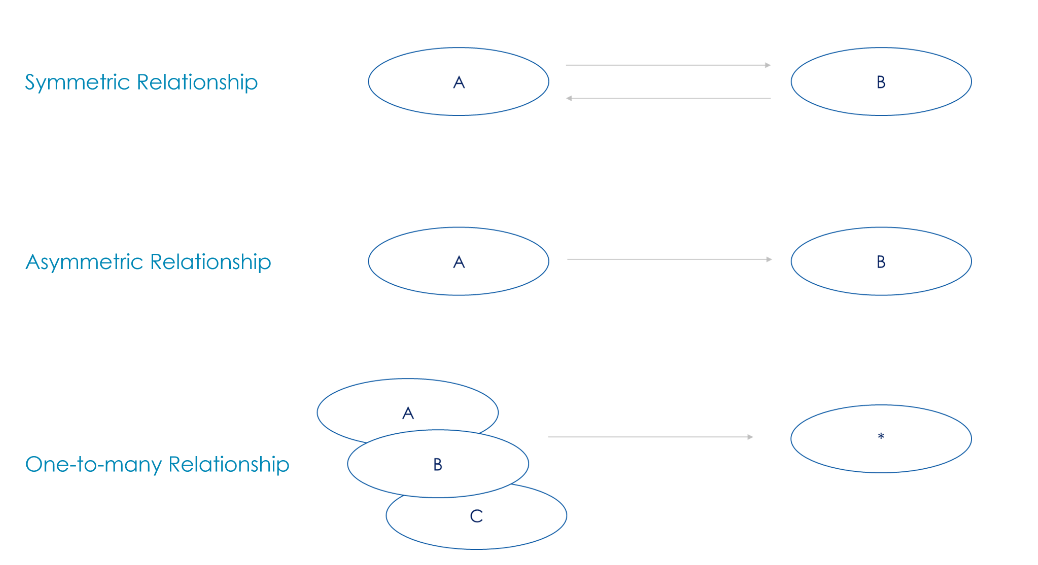
\includegraphics[scale = 0.5]{pictures/cac_moi_quan_he_boi_canh_gioi_han/main.png}

    \caption{Các mối quan hệ bối cảnh bị giới hạn}

\end{figure}

\subsubsection{Mối quan hệ đối xứng (Symmetric Relationship)}

\paragraph{Mô hình riêng biệt (Separate Ways)}

Khi các bối cảnh bị giới hạn có quan hệ riêng biệt, không có sự phụ thuộc. Vì vậy, các bối cảnh bị giới hạn này có ngôn ngữ, mô hình, mục đích độc lập và thực thi riêng biệt. Các nhóm phát triển không phải cộng tác hay phối hợp với nhau từ đó đem lại lợi ích dễ dàng bảo trì và mở rộng hệ thống.

\begin{example} Trong miền     ngân hàng, thẻ tín dụng và khoản vay mua nhà không có mối quan hệ.

    \begin{figure}[H]

        \centering

        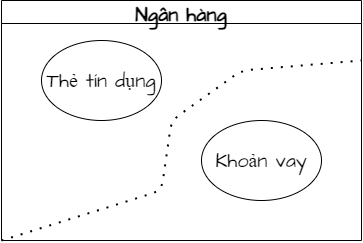
\includegraphics[scale = 0.5]{pictures/mo_hinh_rieng_biet_separate_ways/main.drawio.png}

        \caption{Ví dụ mô hình riêng biệt (Separate Ways)}

    \end{figure}

\end{example}


\paragraph{Mô hình hạt nhân chung (Shared Kernel)}




Trong thực tế, nhiều bối cảnh bị giới hạn phụ thuộc lẫn nhau. Mô hình hợp tác (Partnership) tạo điều kiện cho việc giao tiếp và cộng tác giữa các bối cảnh bị giới hạn phụ thuộc. Tuy nhiên, sự phụ thuộc này dẫn đến mức độ kết hợp cao giữa các nhóm và bối cảnh bị giới hạn, dẫn tới mất đi tính độc lập.

\emph{Lưu ý: Mô hình hợp tác không phải là mô hình của các mẫu chiến lược trong thiết kế huớng miền.}

Để giải quyết vấn đề bối cảnh bị giới hạn phụ thuộc lẫn nhau chúng ta có mô hình hạt nhân chung. Mô hình hạt nhân chung (Shared Kernel) cho phép các bối cảnh bị giới hạn có phần chia sẻ chung và có ranh giới phân định rõ ràng. Từ đó, tách việc quản lí các mô hình hạt nhân chung này một cách độc lập với phần còn lại của bối cảnh bị giới hạn. Khi cần thay đổi mà không phải của mô hình hạt nhân chung thì nhóm sẽ hoạt động độc lập. Thông thường, mô hình hạt nhân chung được hiện thực hóa bằng các thư viện chung. Tuy nhiên, chỉ sử dụng mô hình hạt nhân chung nếu quan hệ của các bối cảnh bị giới hạn nhỏ và ổn định để tránh quan hệ phức tạp và ràng buộc chặt chẽ.



\begin{example} Trong miền vấn đề ngân hàng, thẻ tín dụng và khoản vay mua nhà không có mối quan hệ.

\begin{figure}[H]

\centering

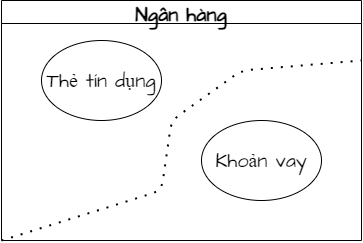
\includegraphics[scale = 0.5]{pictures/mo_hinh_rieng_biet_separate_ways/main.drawio.png}

\caption{Ví dụ mô hình hạt nhân chung (Shared Kernel)}

\end{figure}

\end{example}








\subsubsection{Mối quan hệ bất đối xứng (Asymmetric Relationship)}

% Trong mối quan hệ bất đối xứng, một bối cảnh bị giới hạn có sự phụ thuộc vào một bối cảnh bị giới hạn khác. Mối quan hệ này được mô tả bằng cách gán vai trò cho bối cảnh bị giới hạn :

% \begin{itemize}

% \item \textbf{Bối cảnh bị giới hạn thượng nguồn (Upstream):}

% \begin{itemize}

% \item Bối cảnh bị giới hạn cung cấp cho bối cảnh bị giới hạn khác.

% \item Ký hiệu: U

% \end{itemize}

% \item \textbf{Bối cảnh bị giới hạn hạ lưu (Downstream):}

% \begin{itemize}

% \item Bối cảnh bị giới hạn phụ thuộc vào bối cảnh bị giới hạn khác.

% \item Ký hiệu: D

% \end{itemize}

% \end{itemize}

% \begin{example} Mối quan hệ bất đối xứng giữa bối cảnh bị giới hạn A và bối cảnh bị giới hạn B.

% \begin{itemize}

% \item Bối cảnh bị giới hạn A ràng buộc với bối cảnh bị giới hạn B

% \item Bối cảnh bị giới hạn A đóng vai trò là bối cảnh bị giới hạn hạ lưu (Downstream)

% \item Bối cảnh bị giới hạn B đóng vai trò là bối cảnh bị giới hạn thượng nguồn (Upstream)

% \item Bối cảnh bị giới hạn A có kiến thức về các mô hình trong bối cảnh bị giới hạn B

% \item Bối cảnh bị giới hạn B không có bất kỳ kiến thức nào về mô hình trong bối cảnh bị giới hạn A

% \end{itemize}

% \begin{figure}[H]

% \centering

% 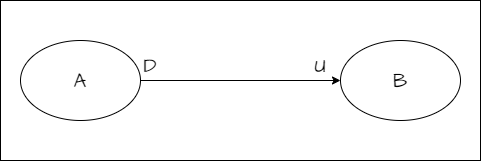
\includegraphics[scale = 0.5]{pictures/moi_quan_he_bat_doi_xung/main.drawio.png}

% \caption{Ví dụ mối quan hệ bất đối xứng}

% \end{figure}

% \end{example}

% % \xxxxxxxxxxxxxxxxxxxxx{Mô hình khách hàng - nhà cung cấp (Customer - Supplier)}

% Mô hình khách hàng - nhà cung cấp (Customer - Supplier) được thể hiện rằng bối cảnh bị giới hạn thượng nguồn đáp ứng nhu cầu của bối cảnh bị giới hạn hạ lưu.

% Khi đó:

% \begin{itemize}

% \item Bối cảnh bị giới hạn thượng nguồn được gọi là nhà cung cấp.

% \item Bối cảnh bị giới hạn hạ lưu được gọi là khách hàng.

% \end{itemize}

% Trong thực tế, nhóm phát triển nhà cung cấp luôn tham khảo ý kiến của nhóm phát triển khách hàng và có bộ kiểm thử để đảm bảo rằng dịch vụ của nhà cung cấp đáp ứng được yêu cầu của khách hàng.

% % \xxxxxxxxxxxxxxxxxxxxx{Mô hình tuân thủ (Conformist)}

% Trong mô hình khách hàng - nhà cung cấp, nếu nhà cung cấp thực hiện tốt yêu cầu thì khách hàng cần tuân thủ chặt chẽ. Mô hình tuân thủ (Conformist) là một mối quan hệ trong đó bối cảnh bị giới hạn hạ lưu áp dụng mô hình, ngôn ngữ chung và các khái niệm của bối cảnh bị giới hạn thượng nguồn.

% Trong mô hình tuân thủ bối cảnh bị giới hạn hạ lưu được ký hiệu là CF.

% %! $VD: - - >

% %! $VD: A - CF - U - B - - >

% %! $VD: A - users(id, name) - B cũng users(id, name) - - >

% % Vẽ lại bản đồ tiếng Việt

% % Vẽ lại bản đồ tiếng Việt

% % Vẽ lại bản đồ tiếng Việt

% % Vẽ lại bản đồ tiếng Việt

% % Vẽ lại bản đồ tiếng Việt

% % Vẽ lại bản đồ tiếng Việt

% % Vẽ lại bản đồ tiếng Việt

% % Vẽ lại bản đồ tiếng Việt

% % Từ bản đồ lấy vi dụ cho các mô hình

% % Từ bản đồ lấy vi dụ cho các mô hình

% % Từ bản đồ lấy vi dụ cho các mô hình

% % Từ bản đồ lấy vi dụ cho các mô hình

% % Từ bản đồ lấy vi dụ cho các mô hình

% % Từ bản đồ lấy vi dụ cho các mô hình

% % Từ bản đồ lấy vi dụ cho các mô hình

% % Từ bản đồ lấy vi dụ cho các mô hình

% % Từ bản đồ lấy vi dụ cho các mô hình

% % Từ bản đồ lấy vi dụ cho các mô hình

% \begin{example} Trong miền vấn đề ngân hàng, thẻ tín dụng và khoản vay mua nhà không có mối quan hệ.

% \begin{figure}[H]

% \centering

% 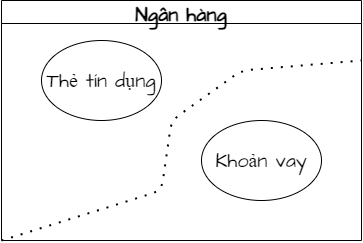
\includegraphics[scale = 0.5]{pictures/mo_hinh_rieng_biet_separate_ways/main.drawio.png}

% \caption{Ví dụ mô hình riêng biệt (Separate Ways)}

% \end{figure}

% \end{example}

% % \xxxxxxxxxxxxxxxxxxxxx{Mô hình chống đổ vỡ (Anti Corruption Layer)}

% Trong mô hình khách hàng - nhà cung cấp, nếu nhà cung cấp có thể thay đổi linh hoạt không đảm bảo đáp ứng nhu cầu của khách hàng thì khách hàng cần có giải pháp xử lí. Mô hình chống đổ vỡ (Anti Corruption Layer) là một mối quan hệ trong đó bối cảnh bị giới hạn hạ lưu sử dụng một lớp để dịch giữa ngôn ngữ của nó và ngôn ngữ của bối cảnh bị giới hạn thượng nguồn.

% Trong mô hình chống đổ vỡ, mỗi bối cảnh bị giới hạn có mô hình riêng biệt và lớp chống đổ vỡ cần kiến thức về mô hình hạ lưu và thượng nguồn để bảo vệ hạ lưu và duy trì tính toàn vẹn.

% %@ Façade

% %@ Adapter

% Trong mô hình chống đổ vỡ bối cảnh bị giới hạn hạ lưu được ký hiệu là ACL.

% % Vẽ lại bản đồ tiếng Việt

% % Vẽ lại bản đồ tiếng Việt

% % Vẽ lại bản đồ tiếng Việt

% % Vẽ lại bản đồ tiếng Việt

% % Vẽ lại bản đồ tiếng Việt

% % Vẽ lại bản đồ tiếng Việt

% % Vẽ lại bản đồ tiếng Việt

% % Vẽ lại bản đồ tiếng Việt

% % Từ bản đồ lấy vi dụ cho các mô hình

% % Từ bản đồ lấy vi dụ cho các mô hình

% % Từ bản đồ lấy vi dụ cho các mô hình

% % Từ bản đồ lấy vi dụ cho các mô hình

% % Từ bản đồ lấy vi dụ cho các mô hình

% % Từ bản đồ lấy vi dụ cho các mô hình

% % Từ bản đồ lấy vi dụ cho các mô hình

% % Từ bản đồ lấy vi dụ cho các mô hình

% % Từ bản đồ lấy vi dụ cho các mô hình

% % Từ bản đồ lấy vi dụ cho các mô hình

% \begin{example} Trong miền vấn đề ngân hàng, thẻ tín dụng và khoản vay mua nhà không có mối quan hệ.

% \begin{figure}[H]

% \centering

% 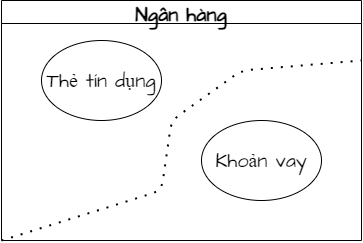
\includegraphics[scale = 0.5]{pictures/mo_hinh_rieng_biet_separate_ways/main.drawio.png}

% \caption{Ví dụ mô hình riêng biệt (Separate Ways)}

% \end{figure}

% \end{example}

\subsubsection{Mối quan hệ 1 - nhiều (One to Many Relationship)}

% % \xxxxxxxxxxxxxxxxxxxxx{Dịch vụ máy chủ mở (Open Host Service)}

% Dịch vụ máy chủ mở (Open Host Service) là nhà cung cấp trong mô hình khách hàng - nhà cung cấp, dịch vụ máy chủ mở hiển thị một API công khai cho các bối cảnh bị giới hạn khác sử dụng chức năng của nhà cung cấp.

% Trong bản đồ bối cảnh, dịch vụ máy chủ mở được ký hiệu là OHS.

% % Vẽ lại bản đồ tiếng Việt

% % Vẽ lại bản đồ tiếng Việt

% % Vẽ lại bản đồ tiếng Việt

% % Vẽ lại bản đồ tiếng Việt

% % Vẽ lại bản đồ tiếng Việt

% % Vẽ lại bản đồ tiếng Việt

% % Vẽ lại bản đồ tiếng Việt

% % Vẽ lại bản đồ tiếng Việt

% % Từ bản đồ lấy vi dụ cho các mô hình

% % Từ bản đồ lấy vi dụ cho các mô hình

% % Từ bản đồ lấy vi dụ cho các mô hình

% % Từ bản đồ lấy vi dụ cho các mô hình

% % Từ bản đồ lấy vi dụ cho các mô hình

% % Từ bản đồ lấy vi dụ cho các mô hình

% % Từ bản đồ lấy vi dụ cho các mô hình

% % Từ bản đồ lấy vi dụ cho các mô hình

% % Từ bản đồ lấy vi dụ cho các mô hình

% % Từ bản đồ lấy vi dụ cho các mô hình

% \begin{example} Trong miền vấn đề ngân hàng, thẻ tín dụng và khoản vay mua nhà không có mối quan hệ.

% \begin{figure}[H]

% \centering

% 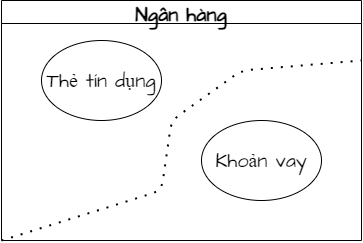
\includegraphics[scale = 0.5]{pictures/mo_hinh_rieng_biet_separate_ways/main.drawio.png}

% \caption{Ví dụ mô hình riêng biệt (Separate Ways)}

% \end{figure}

% \end{example}

% % \xxxxxxxxxxxxxxxxxxxxx{Ngôn ngữ được xuất bản (Published Language)}

% Khi ngôn ngữ chung ở dịch vụ máy chủ mở được các nhóm phát triển trong bối cảnh bị giới hạn hạ lưu chấp nhận. Ngôn ngữ chung này được gọi là ngôn ngữ được xuất bản (Published Language). Ngôn ngữ được xuất bản có lợi ích là tính thống nhất trong hệ thống tuy nhiên cần phân tích kĩ vì nó có thể tạo ra sự nhầm lẫn trong bối cảnh bị giới hạn hạ lưu nào đó.

% Trong bản đồ bối cảnh, ngôn ngữ được xuất bản kết hợp dịch vụ máy chủ mở được ký hiệu là OHS|PL.

% % Vẽ lại bản đồ tiếng Việt

% % Vẽ lại bản đồ tiếng Việt

% % Vẽ lại bản đồ tiếng Việt

% % Vẽ lại bản đồ tiếng Việt

% % Vẽ lại bản đồ tiếng Việt

% % Vẽ lại bản đồ tiếng Việt

% % Vẽ lại bản đồ tiếng Việt

% % Vẽ lại bản đồ tiếng Việt

% % Từ bản đồ lấy vi dụ cho các mô hình

% % Từ bản đồ lấy vi dụ cho các mô hình

% % Từ bản đồ lấy vi dụ cho các mô hình

% % Từ bản đồ lấy vi dụ cho các mô hình

% % Từ bản đồ lấy vi dụ cho các mô hình

% % Từ bản đồ lấy vi dụ cho các mô hình

% % Từ bản đồ lấy vi dụ cho các mô hình

% % Từ bản đồ lấy vi dụ cho các mô hình

% % Từ bản đồ lấy vi dụ cho các mô hình

% % Từ bản đồ lấy vi dụ cho các mô hình

% \begin{example} Trong miền vấn đề ngân hàng, thẻ tín dụng và khoản vay mua nhà không có mối quan hệ.

% \begin{figure}[H]

% \centering

% 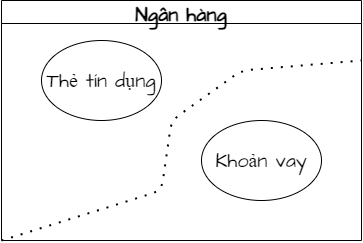
\includegraphics[scale = 0.5]{pictures/mo_hinh_rieng_biet_separate_ways/main.drawio.png}

% \caption{Ví dụ mô hình riêng biệt (Separate Ways)}

% \end{figure}

% \end{example}

% %%%%%%%%%%%%%%%%%%%%%%%%%%%%%%%%%%

% %%%%%%%%%%%%%%%%%%%%%%%%%%%%%%%%%%

% %%%%%%%%%%%%%%%%%%%%%%%%%%%%%%%%%%

% %%%%%%%%%%%%%%%%%%%%%%%%%%%%%%%%%%

% %%%%%%%%%%%%%%%%%%%%%%%%%%%%%%%%%%

% %%%%%%%%%%%%%%%%%%%%%%%%%%%%%%%%%%

% %%%%%%%%%%%%%%%%%%%%%%%%%%%%%%%%%%

% %%%%%%%%%%%%%%%%%%%%%%%%%%%%%%%%%%

% % \section{Áp dụng về các mối quan hệ bối cảnh bị giới hạn}

% %! Hướng dẫn 6/6

% %%%%%%%%%%%%%%%%%%%%%%%%%%%%%%%%%%

% %%%%%%%%%%%%%%%%%%%%%%%%%%%%%%%%%%

% %%%%%%%%%%%%%%%%%%%%%%%%%%%%%%%%%%

% %%%%%%%%%%%%%%%%%%%%%%%%%%%%%%%%%%
